\section{Application}

L'application est séparée en trois parties majeures qui seront détaillées ci-dessous.

\subsection{Données}
Au niveau des données, l'application se base sur un type global qui est un \textit{Problem}. Ce type contient toutes les informations nécessaires à la résolution du problème. Un autre type qui peut être fourni est le \textit{Solution}. En plus de contenir le problème correspondant à la solution, il contient également le résultat obtenu par le solveur. Un fichier contenant la solution est créé automatiquement lorsqu'une solution est trouvée.

Ci-dessous, un exemple de fichier JSON contenant les données d'un problème :

\begin{listing}[H]
    \inputminted{json}{assets/figures/example.json}
    \caption{Exemple de fichier JSON d'un problème}
\end{listing}


La librairie utilisée pour lire le fichier JSON est \textit{Jackson}. Elle permet de lire le fichier JSON et de le convertir en objet Java. L'objet Java est ensuite utilisé par l'application pour créer les différents objets nécessaires à la résolution du problème. Grâce à cette librairie, le mapping entre les données et les objets Java est automatique.

\begin{listing}[H]
    \inputminted{java}{assets/figures/parser.java}
    \caption{Parser JSON}
\end{listing}

La méthode \textit{parseProblem} prend en paramètre le nom du fichier JSON à lire et retourne un objet de type \textit{Problem}. Si le fichier JSON n'est pas trouvé ou qu'il ne respecte pas le format attendu, une exception est levée.

L'application permet de spécifier le fichier JSON à lire via l'interface graphique. Actuellement, il n'est pas possible de modifier les données via l'interface graphique, mais cela était une des fonctionnalités prévues si le temps le permettait.

\begin{figure}[H]
    \centering
    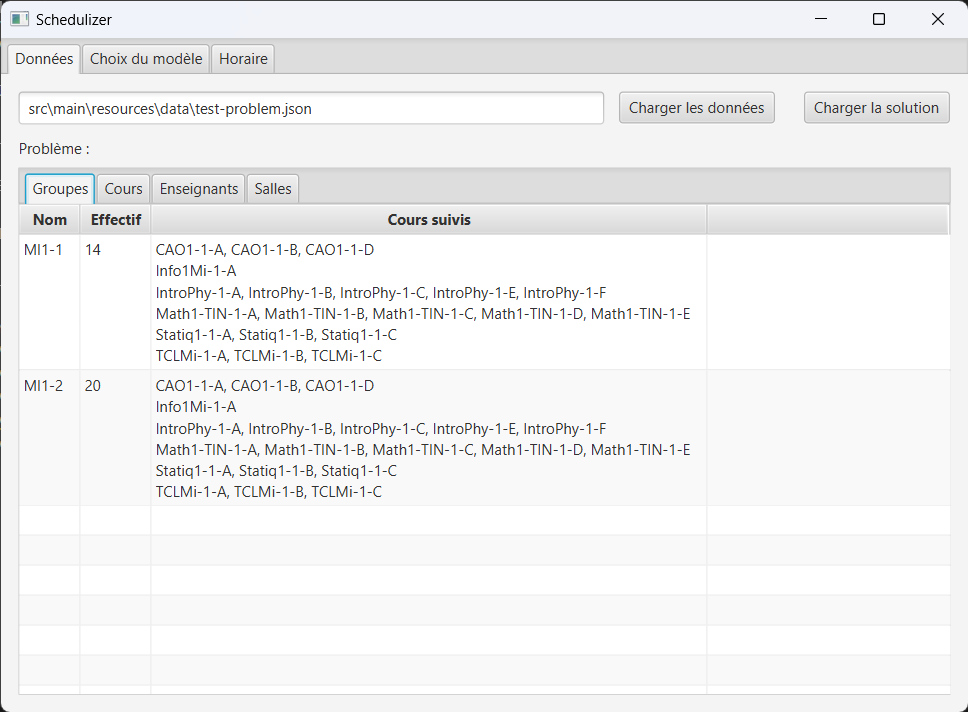
\includegraphics[width=1\textwidth]{./assets/figures/dataWindow.png}
    \caption{Exemple de la fenêtre de données}
\end{figure}

Ci-dessus, un exemple de la fenêtre de données. Les 2 boutons permettent de spécifier si ce que l'on veut lire est un problème ou une solution. Afin de faciliter l'utilisation, un fichier d'exemple est fourni avec l'application et est sélectionné par défaut.

Pour permettre l'affichage de liste d'objets dans les tableaux, il a été nécessaire de créer un type sur mesure représentant une cellule et affichant les listes d'une manière spécifique. Cela permet d'afficher les listes de manière lisible et plus compacte, en plus de faciliter la mise en place d'un système gérant les interactions avec les cellules, tel que cliquer dessus pour modifier la valeur.

\subsection{Contraintes}

La génération de l'horaire est soumise à de multiples contraintes dont certaines sont plus importantes que d'autres. Les contraintes par défaut sont appliquées dès que le modèle est créé. Il est possible d'ajouter des contraintes supplémentaires via l'interface graphique. Une liste de contraintes pré-définies est mise à disposition et il est possible de choisir lesquels nous intéresse via des "Checkbox". Par contre, il n'est pas possible de créer des contraintes personnalisées.

\begin{figure}[H]
    \centering
    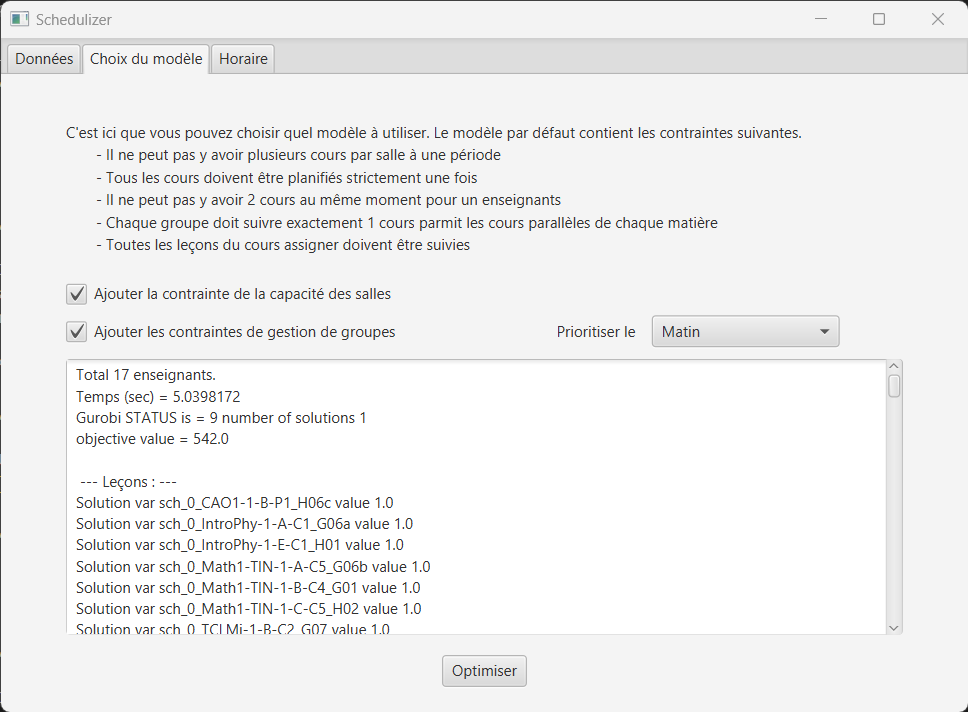
\includegraphics[width=1\textwidth]{./assets/figures/constraintsWindow.png}
    \caption{Exemple de la fenêtre de contraintes}
\end{figure}
\vspace{\baselineskip}

L'application met à disposition un ensemble de contraintes de base qui sont les suivantes :
\begin{itemize}
    \item \textbf{Contrainte de tout les cours planifiés} : tous les cours doivent être planifiés strictement une fois.
    \item \textbf{Contrainte de disponibilité des professeurs} : un professeur ne peut pas donner deux cours en même temps.
    \item \textbf{Contrainte de disponibilité des salles} : une salle ne peut pas être utilisée pour deux cours en même temps.
    \item \textbf{Contrainte des cours suivis} : chaque groupe doit suivre tous les cours lui étant assigné.
    \item \textbf{Contrainte des leçons suivies} : chaque leçon composant un cours doit être suivi par le groupe suivant le cours.
    \item \textbf{Contrainte des cours optionnels (optionnel)} : chaque groupe doit suivre exactement 1 cours parmi les cours parallèles d'une matière.
    \item \textbf{Contrainte de la capacité des salles {optionnel}} : la capacité d'une salle doit être suffisante pour accueillir le ou les groupes suivant le cours.
\end{itemize}
\vspace{\baselineskip}

La contrainte des cours suivis est une contrainte par défaut, mais la contrainte des cours optionnels vient se rajouter par-dessus si elle est sélectionnée. La première va faire en sorte que chaque groupe suis tout les cours qui lui sont assignés. Mais dans les données du problème, il est possible de spécifier des cours optionnels. Dans le cas où la contrainte des cours optionnels ne serait pas activée, le premier cours sera pris par défaut. Dans le cas contraire, le modèle va trouver la solution optimale en assignant à chaque groupe un cours optionnel. De plus, le fait de l'ajouter va rajouter une contrainte supplémentaire qui va nous assurer que lorsqu'un groupe est assigné à un cours, toute les leçons le composant sont également assignées.

L'autre contrainte optionnel (capacité des salles), est relativement simple. Elle va vérifier que la salle est assez grande pour accueillir le ou les groupes suivant le cours. Si ce n'est pas le cas, la contrainte n'est pas respectée et le modèle sera forcé de trouver une autre salle pour ce cours.

Il se peut que le modèle ne trouve pas de solution respectant les contraintes données ou qu'il n'y a pas de solutions du tout. Le cas échéant, un fichier \textit{model.ilp} sera automatiquement généré. Contenu dedans seront toutes les contraintes posant problème. Ce qui permet de rapidement trouver quels points ont empêchés de trouver une solution viable.

Les détails sur l'implémentation mathématique et informatique de ces contraintes sont disponibles dans la section \textit{Modèle}.

\subsection{Affichage}

\begin{figure}[H]
    \centering
    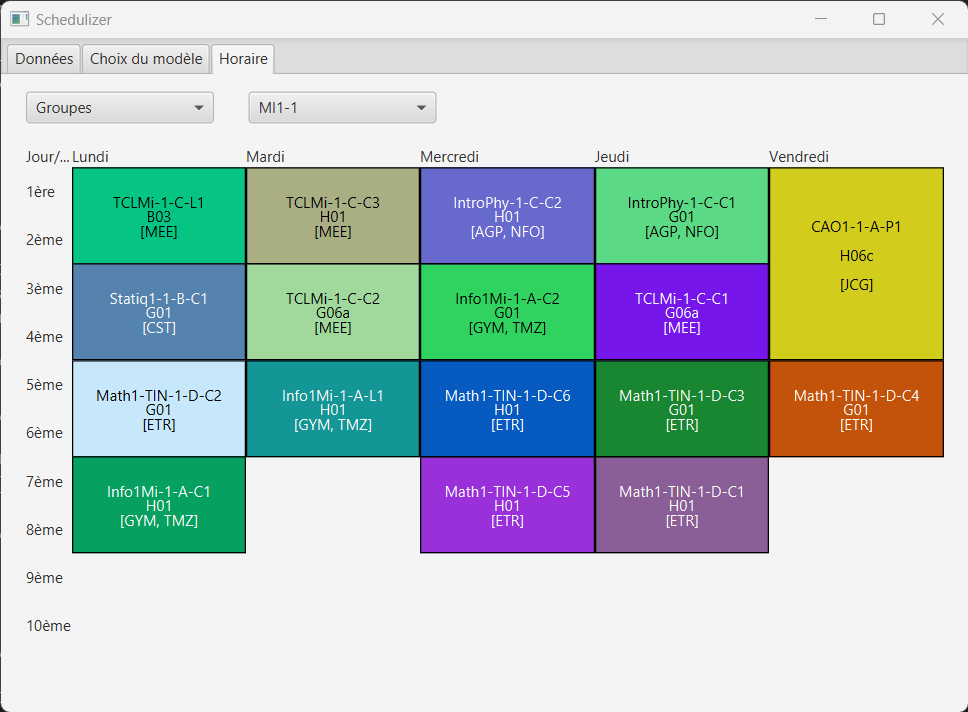
\includegraphics[width=1\textwidth]{./assets/figures/scheduleWindow.png}
    \caption{Exemple de la fenêtre de contraintes}
\end{figure}

Une fois l'horaire généré, il va être possible de l'afficher directement dans l'application. L'affichage est réalisé grâce à la librairie \textit{JavaFX}. Il est possible de choisir quel type d'horaire nous souhaitons afficher, les différents types sont les suivants :

\begin{itemize}
    \item \textbf{Horaire des cours} : affiche où et quand sont planifiées toutes les leçons d'un cours.
    \item \textbf{Horaire des professeurs} : affiche les cours de chaque professeur.
    \item \textbf{Horaire des salles} : affiche les cours de chaque salle.
    \item \textbf{Horaire des groupes} : affiche les cours de chaque groupe.
\end{itemize}

\vspace{\baselineskip}

Chaque case de l'horaire représente une période. Lorsque l'on entre un cours, il faut spécifier la période, le jour, la durée, ainsi que le nom de la leçon. A partir de ces informations, une entrée va être ajoutée à l'horaire. La période et le jour correspondent à la position de l'entrée dans l'horaire. La durée correspond au nombre de périodes que l'entrée va occuper. De plus, la salle ainsi que les professeurs sont récupérés puis affichés avec le nom de la leçon. Pour chaque nouveau cours, une couleur aléatoire est générée et attribuée à l'entrée. Cela permet de différencier les cours plus facilement.